\documentclass[letterpaper,11pt,oneside]{article}
\usepackage[left=0.75in, right=0.5in, bottom=1.25in, top=0.4in]{geometry}
\usepackage{graphicx}
\usepackage{setspace}
\graphicspath{ {/}}
\linespread{1}

\begin{document}
\begin{center}
\textbf{{\large Krupa Sindhu S}}\\
\end{center}
\vspace{-2ex}
\noindent\hrulefill
\vspace{1ex}

\small {\noindent{  {\#154,}} \hfill  {Contact:9148887198}\\
	{7th cross,} \hfill  {Email:krps123450@gmail.com}\\
	{Mahalakshmipuram},\\
	{Bangalore-560086,}\\
	{Karnataka}}

 \hfill 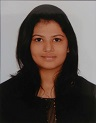
\includegraphics[scale=0.7]{krupa.jpg}\\
 
 \noindent\textbf{{\normalsize  OBJECTIVE}}\\
 \small {Dedicated, energetic and motivated team player seeking an intership position where my potentials will be fully discovered.\\}
 
 \noindent\textbf{{\normalsize  EDUCATION}}\\
 \\
 \begin{tabular}{ |c|c|c|c|c| } 
 	\hline
 	&&&&\\ 
 	\textbf{\large{Examination}} & \textbf{\large{Year of}} & \textbf{\large{Board}} & \textbf{\large{University}} & \textbf{\large{Percentage}} \\
 	& \textbf{Completion} & &  &\textbf{of marks}  \\
 	\hline
 	&&&&\\ 
 	B.E&2020 &R.V. College of & Autonomous  & 9.4\\   
 	(C.S.E)  &  (Pursuing) & Engineering &Affiliated to VTU   &(CGPA: 3 semesters) \\
 	\hline
 	&&&&\\ 
 	XII &2016  & Karnataka State & KMWA P.U.College &  96\% \\
 	&  & & Bengaluru & \\
 	\hline
 	&&&&\\ 
 	X & 2014   & I.C.S.E & Presidency School, & 97.5\% \\
 	&  & & Bengaluru & \\
 	\hline
 \end{tabular}

\vspace{5ex}

\noindent\textbf{{\normalsize PROJECTS}} \begin{enumerate}
	\item 
	\small {\textbf{Planter Bot (December 2017 to March 2018- EYRC-2017,IIT Bombay)}\\\\
		\textbf{Project Objective}\\
		The planter bot traverses different zones in the given arena with the help of image processing techniques
		and depending on the number and type of seedlings detected in each zone, corresponding images are overlayed on the background image.\\
		\textbf{Role and Responsibilities}\\
		Contributed to the algorithm and code of the project\\
		Challenges :Shadow and Glare Removal, Path and Zone Detection , Different image processing techniques for following black and white paths, Image Overlay
		
		\item \textbf{Continuous Care Systems}
		(On-going project in CSE,RVCE in collaboration with Hewlett Packard Enterprise(HPE))\\\\
		\textbf{Project Objective}\\
		Abrupt changes in body conditions and health inspires the need for continuous monitoring and analysis of the human body,especially for patients with long-time illnesses.\\
		Therefore,a coordinated,responsive system with patients and doctors that serves without delay would significantly improve healthcare and enable patients to lead a normal life.\\
		\textbf{Role and Responsibilities}\\
		Ideation of styling the UI for easier recognition of the current condition of the patient being monitored(Dynamic data updation,Regular report generation on the patient side application)\\
		Challenges :Continuous updation of real time data, Getting appropriate sensors for various types of monitoring
	}
	
\end{enumerate}

\vspace{2ex}

\noindent\textbf{{\normalsize  TRAINING AND INTERNSHIP}} \begin{itemize}
	\small {\item 	Completed \textbf{NPTEL} Online Certification on Introduction to Modern Application Development, \textbf{IIT Madras}
		\item	Completed Arduino training conducted by Astra Robotics,RVCE
	}
\end{itemize}
\vspace{2ex}
\noindent\textbf{{\normalsize  TECHNICAL SKILLS}} 

\begin{enumerate}
	\small {\item Programming language : C, Java,Python
		\item Microsoft Office
		\item Boards :  Arduino, Raspberry pi
	}
\end{enumerate}

\end{document}
